\subsection{Main Results}\label{section:main-results}

Table~\ref{tab:main-results}\footnote{We used LexTo (http://www.sansarn.com/lexto), TLTK (https://github.com/attapol/tltk), Multi-cut, and New Multi-cut (https://github.com/PyThaiNLP) to produce non-neural segmentation results} illustrates the evaluation results among the compared models on BERT2010.
%
The best of our models, i.e., OURS, achieved the state-of-the-art performance compared with all the other models.
%
From the statistical significance test results, we concluded that OURS surpasses the state-of-the-art model and the strong baseline models, i.e., Baseline w/ Word and OURS w/o CC w/ Sub.
%
Although using subword units could slightly improve its performance compared with using CCs, OURS outperformed OURS w/o CC w/ Sub on multiple runs as well as performing significantly better at p-level $< 0.05$. 
%
This indicates that CCs are more beneficial than subword units in terms of segmentation performance, moreover, unlike incorporating subword, CCs does not require hyperparameter adjustment.
%
OURS, which uses word and CC information, outperformed Baseline w/ Word, which indicates that CCs can be used to complement linguistic knowledge, particularly word information.
%
We implemented an additional model that replaces the BiLSTM layers with Transformer layers \cite{Vaswani2017} in Baseline. However, the results were noticeably lower than all other models. Note that we used the hyperparameters for the Transformer layers by referring to \citeA{Vaswani2017}.
%
In addition to the non-neural models, every model could not outperform any neural model.
%
However, as for TLTK and New Multi-Cut that incorporate with additional linguistic knowledge, i.e., Syllable and CC, show the benefits over LexTo and Multi-Cut in term of segmentation performance.
%
The results show that incorporating with Syllable obviously boosts Word-F1 score and Bound-F1 while CC could help in improving BIES-F1.

\begin{table}
\centering
\scalebox{0.78}{
\begin{tabular}{llccc}
\hline
\textbf{Model} &
  \textbf{Method} &
  \textbf{\begin{tabular}[c]{@{}c@{}}Word-F1\\ ($\sigma$)\end{tabular}} &
  \textbf{\begin{tabular}[c]{@{}c@{}}BIES-F1\\ ($\sigma$)\end{tabular}} &
  \textbf{\begin{tabular}[c]{@{}c@{}}Bound-F1\\ ($\sigma$)\end{tabular}} \\ \hline
LexTo $^\circ$$^\odot$                   & Dict w/ Longest-matching                & 67.29                     & 84.38                  & 91.32                  \\
TLTK $^\circ$$^\odot$                    & Dict w/ Maximum-collocation w/ Syllable & 74.49                     & 86.00                  & 93.01                  \\
Multi-Cut $^\circ$$^\odot$               & Dict w/ Maximum-matching                & 60.36                     & 83.34                  & 88.95                  \\
New Multi-Cut $^\circ$$^\odot$           & Dict w/ Maximum-matching w/ CC          & 68.63                     & 86.39                  & 91.81                  \\ \hdashline
\cite{Treeratpituk2017}$^\circ$          & LSTM                                    & 92.49                     & 96.53                  & 97.94                  \\
\cite{Chormai2019}$^\circ$               & CNN w/ Syllable                         & 93.79                     & 91.36                  & 98.36                  \\
\cite{Kittinaradorn2019}$^\circ$         & CNN w/ Char-type                        & 95.82                     & 98.17                  & 98.87                  \\
\cite{Lapjaturapit2018}$^\circ$          & BiLSTM w/ CC                            & 96.22                     & 98.43                  & 99.03                  \\
\cite{seeha-etal-2020-thailmcut}$^\circ$ & BiLSTM w/ Char-PTM                      & \underline{97.20}         & 98.80                  & 99.27                  \\ \hline
Baseline                                 & BiLSTM-CRF                              & 96.71 (0.120)             & 98.28 (0.117)          & 99.15 (0.023)          \\
Baseline w/ Word                         & BiLSTM-CRF w/ Word                      & \underline{97.57} (0.003) & 98.94 (0.008)          & 99.35 (0.008)          \\ \hdashline
Baseline w/o BiLSTM w/ BERT              & BERT-CRF                                & 97.18 (0.012)             & 98.77 (0.029)          & 99.24 (0.021)          \\
Baseline w/ BERT w/ Word                 & BERT-BiLSTM-CRF w/ Word                 & 96.79 (0.310)             & 98.65 (0.095)          & 99.15 (0.080)          \\ \hline
OURS                                     & BiLSTM-CRF w/ Word w/ CC                & \textbf{97.67} (0.020)    & \textbf{98.99} (0.005) & \textbf{99.38} (0.006) \\
OURS w/o CC w/ Sub                       & BiLSTM-CRF w/ Word w/ Sub               & \underline{97.60} (0.035)             & 98.96 (0.021)          & 99.35 (0.009)          \\
OURS w/o Word                            & BiLSTM-CRF w/ CC                        & 97.42 (0.020)             & 98.91 (0.012)          & 99.32 (0.007)          \\
OURS Swap                                & BiLSTM-CRF w/ Word w/ CC Swap           & 97.61 (0.010)             & 98.97 (0.012)          & 99.36 (0.008)          \\
OURS w/o CC w/ Sub Swap                  & BiLSTM-CRF w/ Word w/ Sub Swap          & 97.45 (0.041)             & 98.87 (0.046)          & 99.32 (0.024)          \\ \hdashline
OURS w/ BERT                             & BERT-BiLSTM-CRF w/ Word w/ CC           & 97.24 (0.030)             & 98.92 (0.020)          & 99.27 (0.016)          \\
OURS w/ BERT w/o CC w/ Sub               & BERT-BiLSTM-CRF w/ Word w/ Sub          & 97.11 (0.081)             & 98.76 (0.049)          & 99.23 (0.035)          \\ \hline
\end{tabular}}
\caption{Comparison among our models, baselines, and Others on BEST2010. Best score for each metric is indicated in \textbf{bold}. OURS was significantly better than state-of-the-art model Thai word segmentation model, Baseline w/ Word, and OURS w/o CC w/ Sub (\underline{underline} scores) at p-level $< 0.05$ in pairwise comparison. All models were evaluated on basis of same dataset division. The scores were obtained from mean of three runs. OURS w/o CC w/ Sub scores were reported on the basis of best validation performance among various subword vocabulary sizes. $\circ$ and $\odot$ indicate reproduced Thai word-segmentation models, and non-neural Thai word-segmentation models, respectively. $\sigma$ represents Population standard deviation.}
\label{tab:main-results}
\end{table}

\begin{table}
\centering
\scalebox{0.83}{
\begin{tabular}{llccccc}
\hline
\textbf{Model} &
  \textbf{Method} &
  \textbf{Word} &
  \textbf{CC} &
  \textbf{Sub} &
  \textbf{LSTM} &
  \textbf{PTM} \\ \hline
LexTo $^\circ$$^\odot$ &
  Dict w/ Longest-matching &
  \multicolumn{1}{l}{\checkmark} &
  \multicolumn{1}{l}{} &
  \multicolumn{1}{l}{} &
  \multicolumn{1}{l}{} &
  \multicolumn{1}{l}{} \\
TLTK $^\circ$$^\odot$ &
  Dict w/ Maximum-collocation w/ Syllable &
  \multicolumn{1}{l}{\checkmark} &
  \multicolumn{1}{l}{} &
  \multicolumn{1}{l}{} &
  \multicolumn{1}{l}{} &
  \multicolumn{1}{l}{} \\
Multi-Cut $^\circ$$^\odot$ &
  Dict w/ Maximum-matching &
  \multicolumn{1}{l}{\checkmark} &
  \multicolumn{1}{l}{} &
  \multicolumn{1}{l}{} &
  \multicolumn{1}{l}{} &
  \multicolumn{1}{l}{} \\
New Multi-Cut $^\circ$$^\odot$ &
  Dict w/ Maximum-matching w/ CC &
  \multicolumn{1}{l}{\checkmark} &
  \multicolumn{1}{l}{\checkmark} &
  \multicolumn{1}{l}{} &
  \multicolumn{1}{l}{} &
  \multicolumn{1}{l}{} \\\hdashline
\cite{Treeratpituk2017}$^\circ$ &
  LSTM &
   &
   &
   &
  \checkmark &
   \\
\cite{Chormai2019}$^\circ$ &
  CNN w/ Syllable &
   &
   &
   &
   &
   \\
\cite{Kittinaradorn2019}$^\circ$ &
  CNN w/ Char-type &
   &
   &
   &
   &
   \\
\cite{Lapjaturapit2018}$^\circ$ &
  BiLSTM w/ CC &
   &
  \checkmark &
   &
  \checkmark &
   \\
\cite{seeha-etal-2020-thailmcut}$^\circ$ &
  BiLSTM w/ Char-PTM &
   &
   &
   &
  \checkmark &
  \checkmark \\ \hline
Baseline &
  BiLSTM-CRF &
   &
   &
   &
  \checkmark &
   \\
Baseline w/ Word &
  BiLSTM-CRF w/ Word &
  \checkmark &
   &
   &
  \checkmark &
   \\ \hdashline
Baseline w/o BiLSTM w/ BERT &
  BERT-CRF &
   &
   &
   &
   &
  \checkmark \\
Baseline w/ BERT w/ Word &
  BERT-BiLSTM-CRF w/ Word &
  \checkmark &
   &
   &
  \checkmark &
  \checkmark \\ \hline
OURS &
  BiLSTM-CRF w/ Word w/ CC &
  \checkmark &
  \checkmark &
   &
  \checkmark &
   \\
OURS w/o CC w/ Sub &
  BiLSTM-CRF w/ Word w/ Sub &
  \checkmark &
   &
  \checkmark &
  \checkmark &
   \\
OURS w/o Word &
  BiLSTM-CRF w/ CC &
   &
  \checkmark &
   &
  \checkmark &
   \\
OURS Swap &
  BiLSTM-CRF w/ Word w/ CC Swap &
  \checkmark &
  \checkmark &
   &
  \checkmark &
   \\
OURS w/o CC w/ Sub Swap &
  BiLSTM-CRF w/ Word w/ Sub Swap &
  \checkmark &
   &
  \checkmark &
  \checkmark &
   \\ \hdashline
OURS w/ BERT &
  BERT-BiLSTM-CRF w/ Word w/ CC &
  \checkmark &
  \checkmark &
   &
  \checkmark &
  \checkmark \\
OURS w/ BERT w/o CC w/ Sub &
  BERT-BiLSTM-CRF w/ Word w/ Sub &
  \checkmark &
   &
  \checkmark &
  \checkmark &
  \checkmark \\ \hline
\end{tabular}
}
\caption{Comparison of the architectures among our models, baselines, and Others. \checkmark indicates whether Word, CC, Subword, LSTM, and PTM are used in the model.}
\label{tab:main-results-desc}
\end{table}

\subsection{Analysis}

\noindent\textbf{Subword-integration Performance:}
We implemented OURS w/o CC w/ Sub on various vocabulary sizes of subword units, as shown in Table~\ref{tab:subword-results}.
%
The results indicate that the vocabulary size clearly affects subword-integration performance improvement.
%
Specifically, by providing more subword vocabulary to the model, we could consistently increase the overall performance.
%
It may reach the performance of OURS when the subword vocabulary size is enormous.
%
However, it might be difficult to appropriately determine the vocabulary size that will benefit the model.
%
For instance, OURS w/o CC w/Sub with 12,800 subword tokens (OURS w/o CC w/ Sub12800) failed to improve in performance compared with those with 3,200 and 6,400 subword tokens.
%
Thus, the size of subword vocabulary is a crucial parameter that affects the performance for this model.

We chose the best subword-integration model on the basis of validation performance to compare it with OURS, as shown in Table~\ref{tab:main-results}. 
%
Both subword and CC integrations tended to act as an additional filter layer for word-integrated character representations and improve segmentation performance.
%
Yet OURS outperformed OURS w/o CC w/ Sub for every evaluation.
%
We think the main reason is that subword units contain noise while CCs do not.
%
For example, a unit that is included in the subword vocabulary but does not exist in Thai word vocabulary and violates the Thai writing system, e.g., a combination of one Thai vowel followed by one Thai consonant, whereas CCs will not include this type of unit.
% ``\foreignlanguage{thaicjk}{าว}'', which is included in the subword vocabulary, does not exist in Thai word vocabulary and violates the Thai writing system, whereas CCs will not include this type of unit.
%

\begin{table}
\centering
\scalebox{1.0}{
\begin{tabular}{lccc}
\hline
\textbf{Model}                     & \textbf{Word-F1} & \textbf{BIES-F1} & \textbf{Bound-F1} \\ \hline
OURS w/o CC w/ Sub800              & 97.56            & 98.94            & 99.35             \\
OURS w/o CC w/ Sub1600             & 97.59            & 98.96            & 99.36             \\
OURS w/o CC w/ Sub3200             & 97.65            & 98.95            & 99.37             \\
\underline{OURS w/o CC w/ Sub6400} & 97.65            & 98.98            & 99.37             \\
OURS w/o CC w/ Sub12800            & 97.65            & 98.95            & 99.37             \\ \hline
\end{tabular}}
\caption{Results of our subword-integration model (OURS w/o CC w/ Sub) with various subword-vocabulary sizes from 800 to 12,800 tokens. The best result of three runs are reported. \underline{underline} indicates model that obtained best score in validation process.}
\label{tab:subword-results}
\end{table}

\medskip\noindent\textbf{Order-of-integration Performance:}
We compared the performance of our model when the order of attention integrations are swapped.
% 
Table~\ref{tab:main-results} shows that the swapped models decrease segmentation performance compared with their original models, especially the swapped subword-integration model.
%
We argue that subword integration initially adds noise to the character representations, e.g., a subword unit that does not exist in Thai word vocabulary.
%
Therefore, it is difficult for the model to complement such representations in the word-attention integration afterwards. 
%
The swapped CC-integration model slightly decreased in performance compared with subword integration because CC vocabulary consists of smaller units that reflect the Thai writing system and includes no noise information.
%
This indicates that OURS outperformed both swapped models and the word information is the priority knowledge to complement a character representation, whereas fine-grained information, i.e., CCs and subword units, are suitable for use after word information as an additional filter layer.


\noindent\textbf{Pre-trained Model Performance}
In this experiment, we replaced BiLSTM layers with BERT layers for extracting \textit{context character vectors} while we simply extract word- and CC-representation from BERT-embedding layer. 
%
From the results as shown in Table~\ref{tab:main-results}, applying pre-trained BERT model into Baseline could improve segmentation performance on BEST2010.
%
However, the BERT-integrated models that incorporate with additional linguistic knowledge, i.e., Baseline w/ BERT w/ Word, OURS w/ BERT, and OURS w/ BERT w/o CC w/ Sub have been obviously reduced in segmentation performance.
%
We think the main reason is pre-trained BERT model could produce unknown token (UNK) to represent unknown characters or candidate words, CC, subword units, which are not included in BERT vocabulary instead of their own representation. 
%
This can be considered as a limitation of applying pre-trained BERT model for fine-tuning straightforwardly without expanding BERT vocabulary to cover all possible candidate words, CC, and subword units.
%
We expect that segmentation performance has potential to be improved in case of the pre-trained BERT model is pre-trained with the train data beforehand, and the BERT vocabulary is appended with candidate words, CC, and subword units.

Although segmentation performance in our model, i.e., OURS w/ BERT and OURS w/ BERT w/o CC w/ Sub are decreased by integrating with pre-trained BERT model, their results yet outperformed Baseline w/ BERT w/ Word. 
%
This indicates that incorporating pre-trained BERT model with multiple linguistic knowledge, including word-layer, and either CC- or subword-unit layer is useful.
%
By comparing the BiLSTM-based models with the BERT-integrated models, while most of the BiLSTM-based models outperformed their own BERT-integrated versions, only Baseline that cannot outperform Baseline w/o BiLSTM w/ BERT. 


\begin{table}
\centering
\scalebox{0.70}{
\begin{tabular}{llcccc}
\hline
\multirow{2}{*}{\textbf{Model}} &
  \multirow{2}{*}{\textbf{Method}} &
  \multicolumn{2}{c}{\textbf{\textbf{TNHC}}} &
  \multicolumn{2}{c}{\textbf{\textbf{VISTEC}}} \\
 &
   &
  \begin{tabular}[c]{@{}c@{}}\textbf{Char-F1}\\ ($\sigma$)\end{tabular} &
  \begin{tabular}[c]{@{}c@{}}\textbf{Word-F1}\\ ($\sigma$)\end{tabular} &
  \begin{tabular}[c]{@{}c@{}}\textbf{Char-F1}\\ ($\sigma$)\end{tabular} &
  \begin{tabular}[c]{@{}c@{}}\textbf{Word-F1}\\ ($\sigma$)\end{tabular} \\ \hline
LexTo $^\circ$$^\odot$ &
  Dict w/ Longest-matching &
  88.10 &
  69.92 &
  87.54 &
  70.43 \\
TLTK $^\circ$$^\odot$ &
  Dict w/ Maximum-collocation w/ Syllable &
  86.95 &
  71.81 &
  88.66 &
  76.73 \\
Multi-Cut $^\circ$$^\odot$ &
  Dict w/ Maximum-matching &
  83.96 &
  67.62 &
  84.52 &
  64.41 \\
New Multi-Cut $^\circ$$^\odot$ &
  Dict w/ Maximum-matching w/ CC &
  88.56 &
  70.32 &
  88.75 &
  73.37 \\ \hdashline
\cite{limkonchotiwat-etal-2020-domain}$^\bullet$ &
  SE-DC (Stack Ensemble) &
  95.2 &
  84.1 &
  - &
  - \\
\cite{limkonchotiwat-etal-2021-handling}$^\circ$ &
  DSE-DC (Deep Stack Ensemble) &
  95.71 &
  85.74 &
  95.07 &
  88.48 \\ \hline
Baseline &
  BiLSTM-CRF &
  98.17 (0.052) &
  95.91 (0.028) &
  96.81 (0.016) &
  91.70 (0.041) \\
Baseline w/ Word &
  BiLSTM-CRF w/ Word &
  \underline{98.39} (0.051) &
  96.40 (0.163) &
  97.09 (0.029) &
  92.42 (0.067) \\ \hdashline
Baseline w/o BiLSTM w/ BERT &
  BERT-CRF &
  98.06 (0.041) &
  95.55 (0.037) &
  97.10 (0.020) &
  92.23 (0.020) \\
Baseline w/ BERT w/ Word &
  BERT-BiLSTM-CRF w/ Word &
  98.31 (0.035) &
  95.46 (0.040) &
  97.04 (0.016) &
  92.19 (0.008) \\ \hline
OURS &
  BiLSTM-CRF w/ Word w/ CC &
  98.54 (0.016) &
  \textbf{96.65} (0.028) &
  \textbf{97.18} (0.012) &
  \textbf{92.65} (0.016) \\
OURS w/o CC w/ Sub &
  BiLSTM-CRF w/ Word w/ Sub &
  \underline{98.41} (0.021) &
  96.39 (0.032) &
  97.04 (0.016) &
  92.27 (0.008) \\ \hdashline
OURS w/ BERT &
  BERT-BiLSTM-CRF w/ Word w/ CC &
  \textbf{98.63} (0.016) &
  96.36 (0.023) &
  97.10 (0.012) &
  92.40 (0.008) \\
OURS w/ BERT w/o CC w/ Sub &
  BERT-BiLSTM-CRF w/ Word w/ Sub &
  98.03 (0.042) &
  94.71 (0.030) &
  96.92 (0.074) &
  92.09 (0.084) \\ \hline
\end{tabular}}
\caption{Comparison among our models and domain-adaptation models on TNHC and VISTEC datasets. Best score for each metric is indicated in \textbf{bold}. The scores from the baseline ans our models were obtained from mean of three runs. OURS was significantly better than Baseline w/ Word and OURS w/o CC w/ Sub (\underline{underline} scores) at p-level $< 0.05$. $\bullet$ indicates reported score from their work. $^\circ$ and $\odot$ indicate reproduced score from neural models and reproduced score from non-neural model. We obtained the results from OSKUT by reproducing their official trained models (https://github.com/mrpeerat/OSKut). $\sigma$ represents Population standard deviation.}
\label{tab:domain-adapt-results}
\end{table}

\noindent\textbf{Comparison with Thai Domain-adaption Models}
To evaluate our models on additional datasets, we compared them with the recent works that focus on the domain-adaptation scenarios on specific datasets, including TNHC and VISTEC. 
 %
The baseline and proposed models were evaluated in an in-domain scenario, i.e., the models were trained on targeted domain training data and evaluated on target domain test data. 
%
For reference, the results of the previous models \cite{limkonchotiwat-etal-2020-domain,limkonchotiwat-etal-2021-handling} trained in a domain adaptation scenario (models were trained using both source and target domain training data) were reported.
%
Concretely, we simply performed our model on the basis of training, validation, and test splits for TNHC and VISTEC.
%
Table~\ref{tab:domain-adapt-results}\footnote{The DSE-DC method from \citeA{limkonchotiwat-etal-2021-handling} was performed on the same dataset division with their official model from https://github.com/mrpeerat/OSKut.} shows the results among our models and domain-adaptation models in character-level- and word-level-evaluation as in the previous work \cite{limkonchotiwat-etal-2020-domain,limkonchotiwat-etal-2021-handling}. 
%
OUR and OUR w/ BERT surpassed every domain-adaptation works as well as outperforming every reproduced models.
%
Specifically, as the tendency of the main results in Section \ref{section:main-results}, OURS was statistically significant better than OURS w/o CC w/ Sub at p-level $p < 0.05$.
%
Moreover, OURS could outperform OURS w/o CC w/ Sub on multiple runs.
%
This emphasizes the benefits of using CCs over subword units.
%
Although we reproduced \citeA{limkonchotiwat-etal-2021-handling} from their original repository, the reproduced results were lower than their reported scores by 3.4 word-F1 scores on TNHC, 2.29 - 4.43 char/word-F1 scores on VISTEC.
%
As for the results of the non-neural models, it shows the same tendency as in Section \ref{section:main-results}, i.e., every non-neural model could not outperform any neural models.
%
In addition, among the non-neural models, the results also show the same direction that using additional knowledge, i.e., syllable and CC, in TLTK and New Multi-Cut could improve segmentation performance.
%
Specifically, by incorporating syllable, TLTK shows outstanding scores on Word-F1 while New Multi-Cut that incorporates with CC could perform well on Char-F1. 

\medskip\noindent\textbf{Case Study:}\label{section:case-study}
Figure~\ref{fig:case-study} shows examples of segmentation results among four models, i.e., Baseline, Baseline /w Word, OURS, and OURS w/o CC w/ Sub.
%
OURS could perfectly segment the example sentence; however, the other models yielded incorrect results. 
%
Specifically, the \textcolor{red}{\underline{underlined word}} violates the Thai writing system by combining the two consonants in the word
%
We think that CC integration filters this type of violation out of the word-integrated character representations, enabling OURS to outperform the other models.
%
 
\begin{figure}
    \centering
    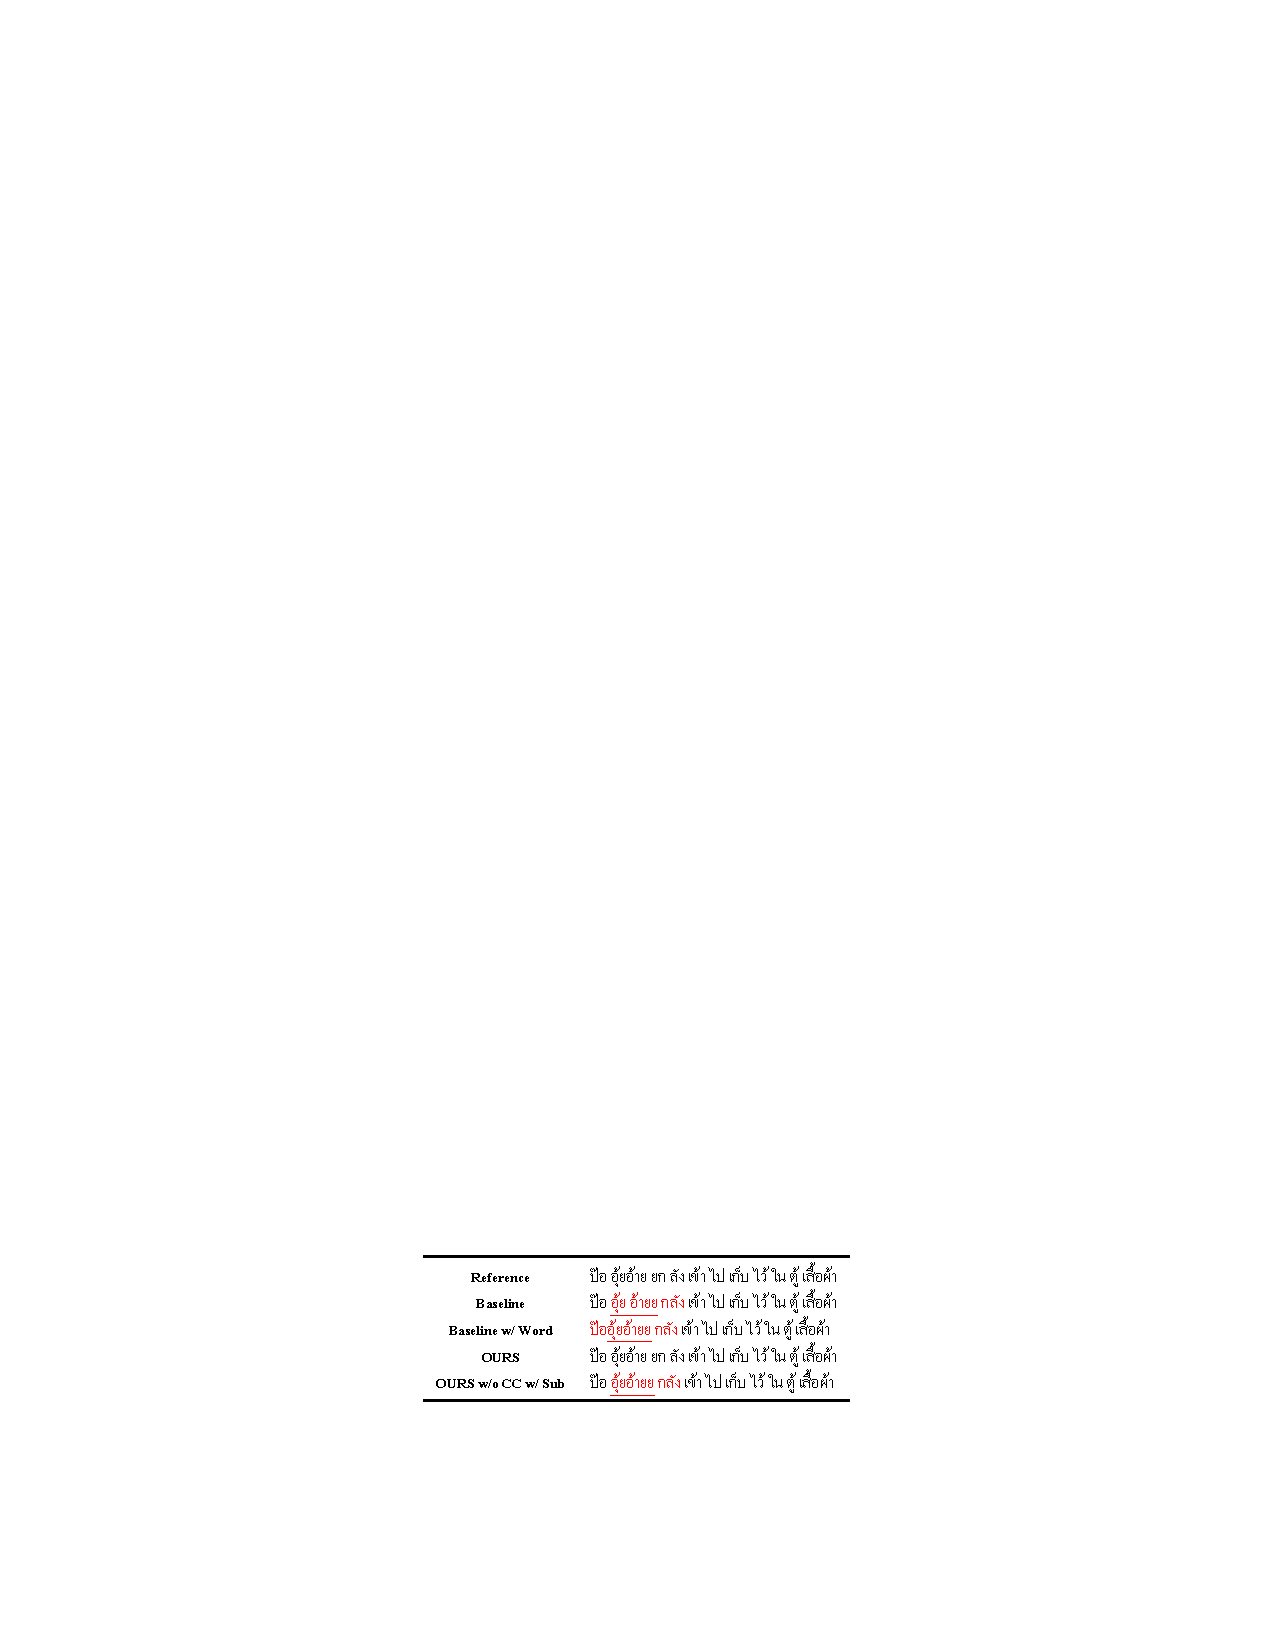
\includegraphics[width=0.6\textwidth]{figures/fig-case-study.pdf}
    \hspace{\textwidth}
    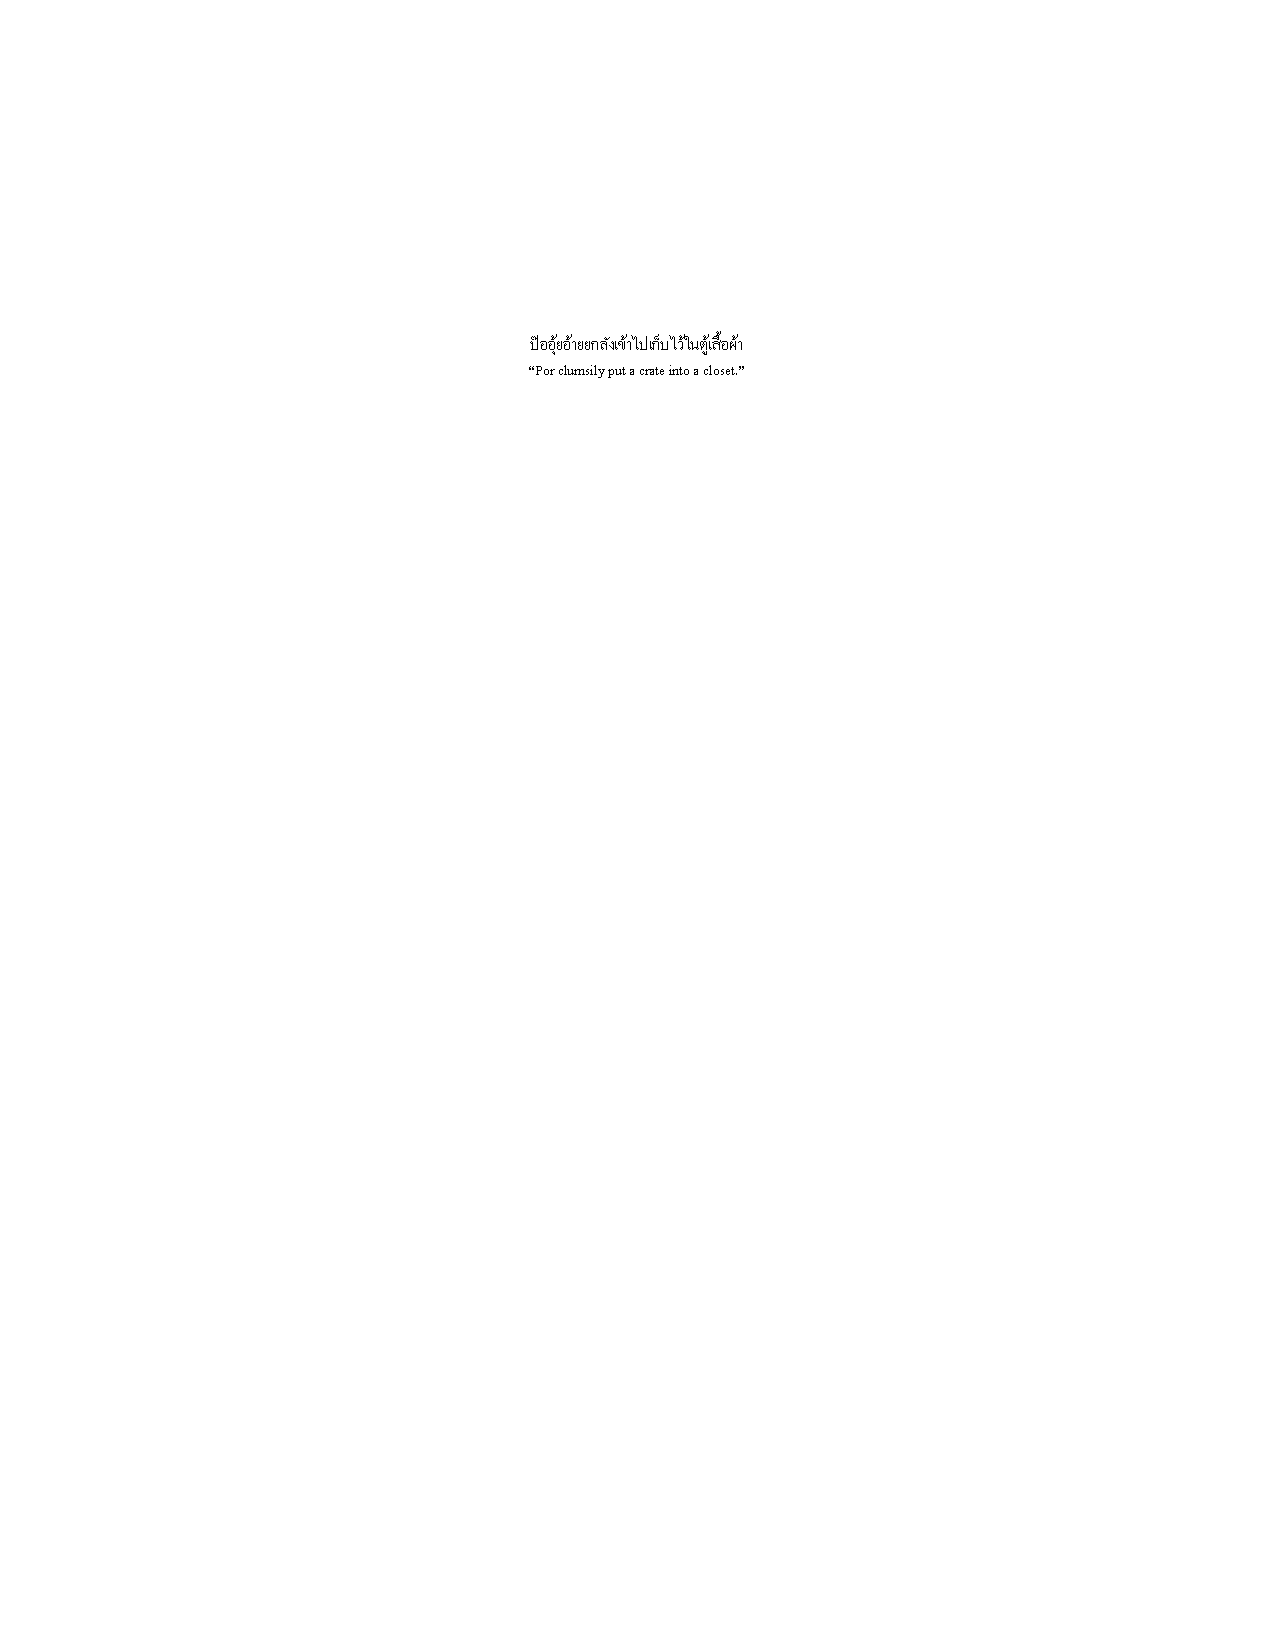
\includegraphics[width=0.35\textwidth]{figures/fig-case-study-tran.pdf}
    \caption{Examples of segmentation results among baseline models and our models. Ground-truth segmentation result is indicated as ``Reference'' and incorrect segmentation results are in \textcolor{red}{red}. \underline{underline} indicates segmentation results that violate Thai writing system.}
    \label{fig:case-study}
\end{figure}